\section{增广拉格朗日法与交替方向乘子法}

本节引入增广拉格朗日函数的概念,分析增广拉格朗日法\cite{1976AugLagrange}与交替方向乘子法\cite{1975ADMMBook},并使用两种方法求解具体的凸优化问题。

\subsection{凸优化模型}

考虑带约束条件的凸优化问题

\begin{equation}\label{eq_admm_1}
    \begin{split}
        &\min\limits_{\bm{x}\in \mathbb{R}^{n}} f(\bm{x}) \\
        &\mathrm{s. t.} \quad\quad \bm{Ax} = \bm{b}
    \end{split}
\end{equation}

其中,$f(x)$是一个连续凸函数,这样的问题一般可以由增广拉格朗日法求解。

而对于如下的约束凸优化问题

\begin{equation}\label{eq_admm_2}
    \begin{split}
        &\min\limits_{\bm{x}\in \mathbb{R}^{n}} f(\bm{x}) := f_{1}(\bm{x}) + f_{2}(\bm{x}) \\
        &\mathrm{s. t.} \quad\quad \bm{A_{1}x_{1}} + \bm{A_{2}x_{2}} = \bm{b} 
    \end{split}
\end{equation}

其中,$f_{1}(\bm{x}), f_{2}(\bm{x})$都是适当的闭凸函数,同时$f(\bm{x})$可以被分解成两个分离的部分$f_{1}(\bm{x})$和$f_{2}(\bm{x})$,但是这两部分被线性约束结合在一起,这样的问题可以由交替方向乘子法求解。
通过对该问题应用交替方向乘子法求解,可以分别更新$\bm{x}_{1}$和$\bm{x}_{2}$的参数,提高了并行计算的效率。

\subsection{增广拉格朗日函数}

在拉格朗日函数的基础上,增加二次罚函数,可以得到增广拉格朗日函数

\begin{equation}\label{eq_admm_3}
    L_{\beta}(x, \lambda) = f(x) + \sum_{i=1}^{m}\lambda_{i} c_{i}(x) + \frac{\beta}{2}\sum_{i=1}^{m}c_{i}^{2}(x),
\end{equation}

其中,式中的$\beta$称为罚因子,$c_{i}(x), i=1, 2, \cdots, m$表示惩罚项。

特别地,当约束关系是线性的时候,即上式中的惩罚项$c(\bm{x})=\bm{Ax}-\bm{b}$时,可以得到增广拉格朗日函数

\begin{equation}\label{eq_admm_4}
    L_{\beta}(\bm{x}, \lambda) = f(\bm{x}) - \lambda^{T}(\bm{Ax}-\bm{b})+\frac{\beta}{2}\|\bm{Ax}-\bm{b}\|_{2}^{2}.
\end{equation}

考虑增广拉格朗日函数\ref{eq_admm_3},使$L_{\beta}(x, \lambda)$值最小的点$x^{k+1}$满足\cite{2016ADMM}

\begin{equation*}
    \nabla_{x} L_{\beta}(x^{k+1}, \lambda^{k}) = \nabla f(x^{k+1}) + \sum_{i=1}^{m} (\lambda_{i}^{k}+\beta c_{i}(x^{k+1})) \nabla c_{i}(x^{k+1}) = 0.
\end{equation*}

因此,根据上式可以得到,对于凸优化问题\ref{eq_admm_1},存在最优解$x^{*}$与最优乘子$\lambda^{*}$,有

\begin{equation}
    \nabla f(x^{*}) + \sum_{i=1}^{m}\lambda_{i}^{*}\nabla c_{i}(x^{*}) = 0.
\end{equation}

\subsection{增广拉格朗日法}

对于凸优化问题\ref{eq_admm_1}即

\begin{equation*}
    \begin{split}
        &\min\limits_{\bm{x}\in \mathbb{R}^{n}} f(\bm{x}) \\
        &\mathrm{s. t.} \quad\quad \bm{Ax} = \bm{b}
    \end{split}
\end{equation*}

使用一般的增广拉格朗日函数\ref{eq_admm_3},增广拉格朗日法有如下的迭代格式

\begin{equation}\label{eq_admm_5}
    \begin{cases}
        \bm{x}^{k+1} &= \mathop{\mathrm{argmin}}\limits_{\bm{x}\in \mathbb{R}^{n}} L_{\beta_{k}}(\bm{x}^{k}, \lambda^{k}) ; \\
        \lambda^{k+1} &= \lambda^{k} + \beta_{k} c(x^{k+1}) .
    \end{cases}
\end{equation}

其中,$\bm{x}^{k+1}$表示第$k+1$次迭代的结果,同样地,$\beta_{k}$表示第$k$次迭代的罚因子,参数的值可以在每次迭代中进行更新。

结合迭代公式\ref{eq_admm_5}与初始化设置,可以将增广拉格朗日法总结为如下算法。

\begin{algorithm}\label{alg_admm_1}
    \SetKwInOut{Input}{输入}\SetKwInOut{Output}{输出}

    \SetAlgoLined
    \Input{$f(\bm{x})$与其增广拉格朗日函数$L_{\beta_{k}}(\bm{x}^{k}, \lambda^{k})$,初始化设置$k=0$,并且给定罚因子的更新常数$\rho > 0$}
    \Output{最优解$\bm{x}^{*}$与最优乘子$\lambda^{*}$}

    \While{未收敛} {
        $\bm{x}^{k+1} = \mathop{\mathrm{argmin}}\limits_{\bm{x}\in \mathbb{R}^{n}} L_{\beta_{k}}(\bm{x}^{k}, \lambda^{k})$
        
        $\lambda^{k+1} = \lambda^{k} + \beta_{k} c(\bm{x}^{k+1})$

        $\beta_{k+1} = \rho \beta_{k}$
    }
    \caption{增广拉格朗日法}
\end{algorithm}

\subsection{交替方向乘子法}

对于凸优化问题\ref{eq_admm_2}即

\begin{equation*}
    \begin{split}
        &\min\limits_{\bm{x}\in \mathbb{R}^{n}} f(\bm{x}) := f_{1}(\bm{x}) + f_{2}(\bm{x}) \\
        &\mathrm{s. t.} \quad\quad \bm{A_{1}x_{1}} + \bm{A_{2}x_{2}} = \bm{b} 
    \end{split}
\end{equation*}

由于其目标函数可以被两个线性约束分离,因此适用于交替方向乘子法求解。

首先,注意到这里的约束条件都是线性的,因此由增广拉格朗日函数\ref{eq_admm_4},可以得到

\begin{equation}
    L_{\beta}(\bm{x_{1}, x_{2}}, \lambda) = f_{1}(\bm{x_{1}}) + f_{2}(\bm{x_{2}}) - \lambda^{T}(\bm{A_{1}x_{1} + A_{2}x_{2}-b} + \frac{\beta}{2}\|\bm{A_{1}x_{1} + A_{2}x_{2}-b}\|_{2}^{2}).
\end{equation}

由上式可以进一步使用增广拉格朗日法得到迭代格式

\begin{equation}
    \begin{cases}
        \bm{x_{1}^{k+1}, x_{2}^{k+1}} &= \mathop{\mathrm{argmin}}\limits_{\bm{x_{1}, x_{2}}} L_{\beta}(\bm{x_{1}^{k}, x_{2}^{k}}, \lambda^{k}); \\
        \lambda^{k+1} &= \lambda^{k} - \beta (\bm{A_{1}x_{1}^{k+1} + A_{2}x_{2}^{k+1} - b}).
    \end{cases}
\end{equation}

注意到上式对于变量$\bm{x_{1}, x_{2}}$的迭代格式与增广拉格朗日法不同的地方在于,上式同时更新了两个变量$\bm{x_{1}}$和$\bm{x_{2}}$,这对于计算求解而言增加了复杂度,因此交替方向乘子法将两个变量分开求解,这样可以充分提升计算效率,下面给出交替方向乘子法的迭代格式

\begin{equation}\label{eq_admm_6}
    \begin{cases}
        \bm{x_{1}^{k+1}} &= \mathop{\mathrm{argmin}}\limits_{\bm{x_{1}}} L_{\beta}(\bm{x_{1}^{k}, x_{2}^{k}}, \lambda^{k}) ; \\
        \bm{x_{2}^{k+1}} &= \mathop{\mathrm{argmin}}\limits_{\bm{x_{2}}} L_{\beta}(\bm{x_{1}^{k+1}, x_{2}^{k}}, \lambda^{k}) ; \\
        \lambda^{k+1} &= \lambda^{k} - \beta (\bm{A_{1}x_{1}^{k+1} + A_{2}x_{2}^{k+1} - b}).
    \end{cases}
\end{equation}

通过交替求解两个变量$\bm{x_{1}}$和$\bm{x_{2}}$的极小,可以交替对其进行更新,并在完成两个变量的更新后,再利用更新后的值对$\lambda$进行更新。

结合迭代公式\ref{eq_admm_6}与初始化设置,可以将交替方向乘子法\cite{2017ADMM}总结为如下算法

\begin{algorithm}\label{alg_admm_2}
    \SetKwInOut{Input}{输入}\SetKwInOut{Output}{输出}

    \SetAlgoLined
    \Input{$f(\bm{x}):=f_{1}(\bm{x})+f_{2}(\bm{x})$与其增广拉格朗日函数$L_{\beta_{k}}(\bm{x_{1}^{k}, x_{2}^{k}}, \lambda^{k})$,初始化设置$k=0$,并且给定罚因子的更新常数$\rho > 0$}
    \Output{最优解$\bm{x_{1}}^{*}, \bm{x_{2}}^{*}$与最优乘子$\lambda^{*}$}

    \While{未收敛} {
        $\bm{x_{1}^{k+1}} = \mathop{\mathrm{argmin}}\limits_{\bm{x_{1}}} L_{\beta}(\bm{x_{1}^{k}, x_{2}^{k}}, \lambda^{k})$  \\        
        
        $\bm{x_{2}^{k+1}} = \mathop{\mathrm{argmin}}\limits_{\bm{x_{2}}} L_{\beta}(\bm{x_{1}^{k+1}, x_{2}^{k}}, \lambda^{k})$  \\

        $\lambda^{k+1} = \lambda^{k} - \rho \beta (\bm{A_{1}x_{1}^{k+1} + A_{2}x_{2}^{k+1} - b})$
    }
    \caption{交替方向乘子法}
\end{algorithm}

\subsection{应用}

以Lasso问题为例,使用交替方向乘子法求解该问题。

\begin{problem}
    求解Lasso问题,即求
    \begin{equation}
        \mathop{\mathrm{min}}\limits_{\bm{x}} f(\bm{x}) := \frac{1}{2}\|\bm{A} \bm{x}-\bm{b}\|_{2}^{2} + \mu\|\bm{x}\|_{1}.
    \end{equation}
\end{problem}

\begin{solution}
    首先,引入变量$\bm{x_{1}}$和变量$\bm{x_{2}}$,使该问题转化成求解

    \begin{equation}
        \begin{split}
            &\mathop{\mathrm{min}}\limits_{\bm{x_{1}, x_{2}}\in \mathbb{R}^{n}} f(\bm{x}) := \frac{1}{2}\|\bm{A} \bm{x_{1}}-\bm{b}\|_{2}^{2} + \mu\|\bm{x_{2}}\|_{1} \\
            &\mathrm{s. t.} \bm{x_{1}} = \bm{x_{2}}
        \end{split}
    \end{equation}

    这样,由线性约束关系可以将目标函数$f(\bm{x})$分解为$f_{1}(\bm{x}) = \frac{1}{2}\|\bm{A} \bm{x_{1}}-\bm{b}\|_{2}^{2}$和$f_{2}(\bm{x}) = \mu\|\bm{x_{2}}\|_{1}$

    于是,可以由增广拉格朗日函数\ref{eq_admm_4}得到,

    \begin{equation*}
        L_{\beta}(\bm{x_{1}}, \bm{x_{2}}, \lambda) = \frac{1}{2} \|\bm{Ax_{1}-b}\|_{2}^{2} + \mu \|\bm{x_{2}}\|_{1} - \lambda^{T}(\bm{x_{1}-x_{2}}) + \frac{\beta}{2} \|\bm{x_{1}-x_{2}}\|_{2}^{2}.
    \end{equation*}

    进一步由迭代公式\ref{eq_admm_5}可以得到

    \begin{equation}
        \begin{cases}
            \bm{x_{1}^{k+1}} &= \mathop{\mathrm{argmin}}\limits_{\bm{x_{1}}} \{ \frac{1}{2}\|\bm{Ax_{1}^{k}}-\bm{b}\|_{2}^{2} + \frac{\beta}{2}\|\bm{x^{k}} - \bm{x_{2}^{k}} -\frac{\lambda^{k}}{\beta}\|_{2}^{2} \} \\
                             &= (\bm{A^{T}A}+\beta\bm{I})^{-1}(\bm{A^{T}b} + \beta\bm{x_{2}^{k}} - \lambda^{k}) ; \\
            \bm{x_{2}^{k+1}} &= \mathop{\mathrm{argmin}}\limits_{\bm{x_{2}}} \{ \mu\|\bm{x_{2}^{k}}\|_{1} + \frac{\beta}{2} \|\bm{x_{2}^{k}}-\bm{x_{1}^{k+1}}+\frac{\lambda^{k}}{\beta}\|_{2}^{2}\} \\
                             &= \mathop{\mathrm{prox_{\frac{\mu}{\beta}\|\cdot\|_{1}}}}(\bm{x_{1}^{k+1}} + \frac{\lambda^{k}}{\beta}) ; \\
            \lambda^{k+1} &= \lambda^{k} + \beta(\bm{x_{1}^{k+1}-\bm{x_{2}^{k+1}}}).
        \end{cases}
    \end{equation}

    使用Python对该问题求解,可以得到结果如图\ref{figure_admm}所示,代码在附录中给出。其中,beta, lambda和rho分别同算法\ref{alg_admm_2}中的$\beta, \lambda, \rho$。可以看出当$\lambda=1$时,不论$\beta$和$\rho$取值如何,都能表现出较好的收敛效果;当$\beta$取值较大时,收敛速度显著提高。
    \begin{figure}[hbtp]
        \centering
        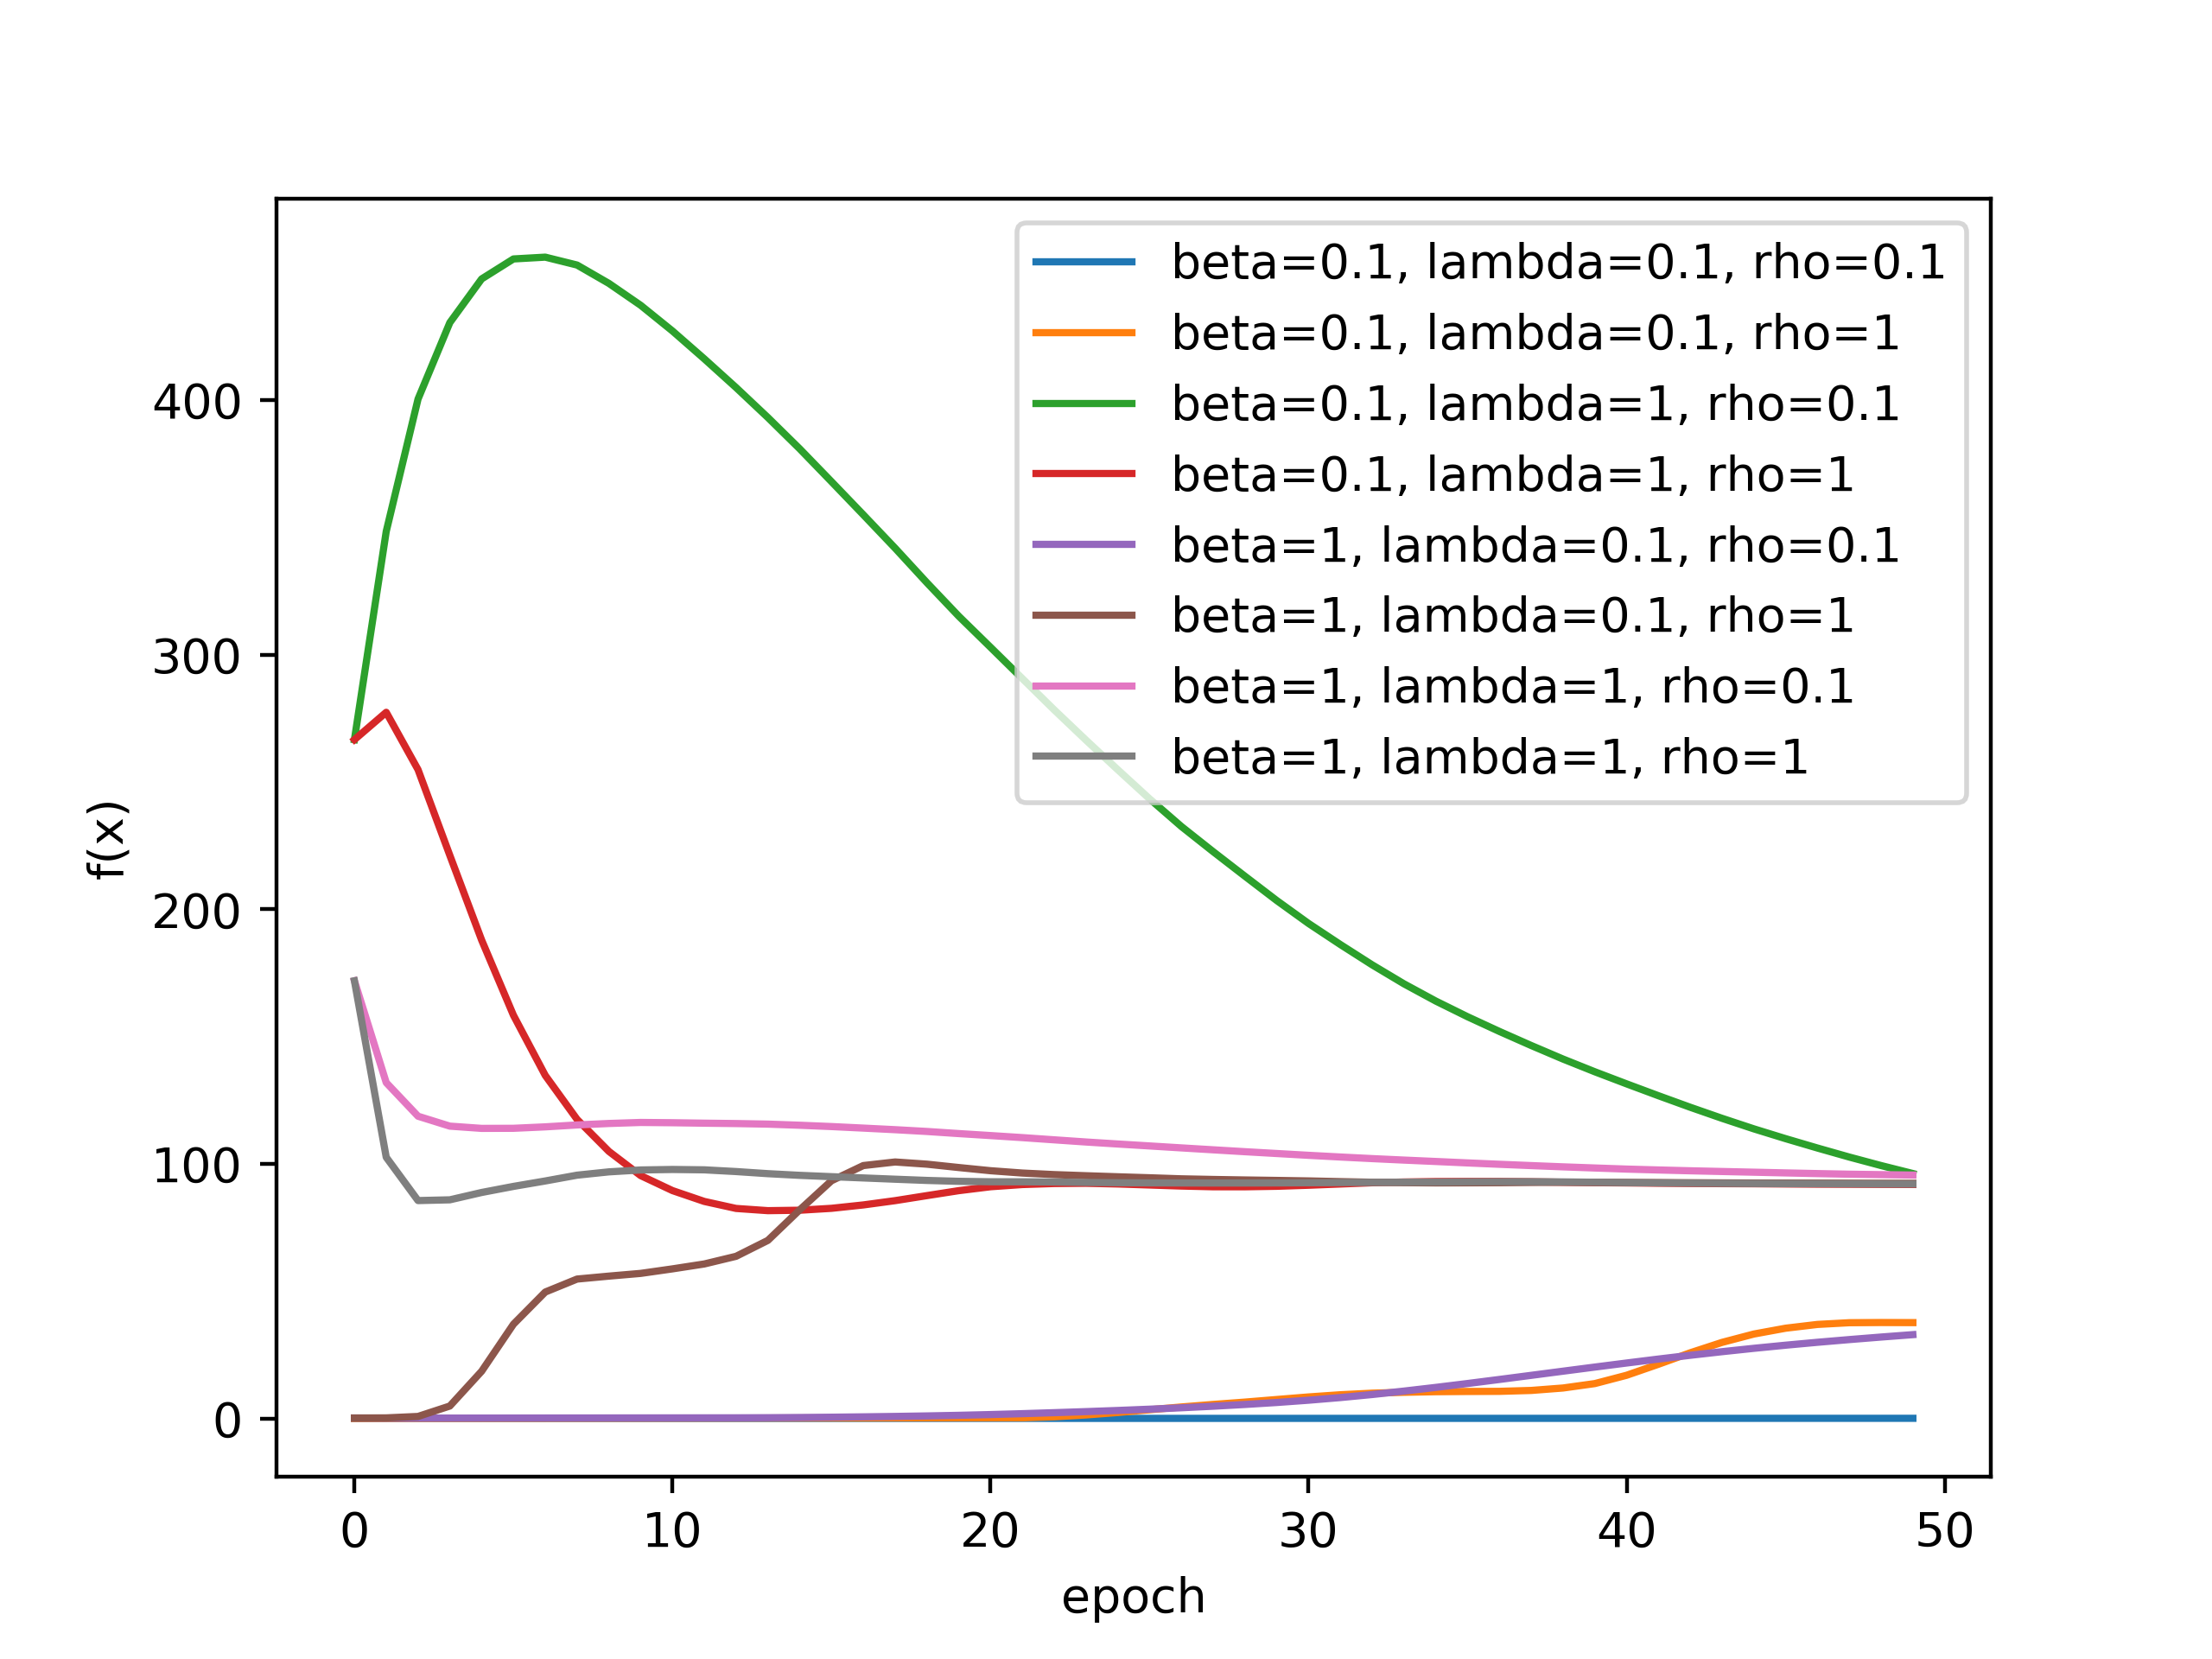
\includegraphics[width=150mm]{./Figures/admm.png}
        \caption{Python实现交替方向乘子法求解Lasso问题}
        \label{figure_admm}
    \end{figure}
\end{solution}